\documentclass{article}
\usepackage{geometry}
\usepackage{amsmath}
\usepackage{color}
\usepackage{xcolor}
\usepackage{amssymb}
\usepackage{listings}
\usepackage{xcolor}
\usepackage{graphicx} %插入图片的宏包
\usepackage{float} %设置图片浮动位置的宏包
\usepackage{subfigure} %插入多图时用子图显示的宏包
\usepackage{cite}
\usepackage{booktabs}
\usepackage{subfigure}
\usepackage{appendix}
\usepackage{pythonhighlight}
\usepackage{authblk}
\usepackage{hyperref}
\definecolor{keywordcolor}{rgb}{0.8,0.1,0.5}
\definecolor{mygreen}{rgb}{0,0.6,0}
\definecolor{mygray}{rgb}{0.5,0.5,0.5}
\definecolor{mymauve}{rgb}{0.58,0,0.82}
\lstset{frame=tb,
  language=Python,
  aboveskip=3mm,
  belowskip=3mm,
  showstringspaces=false,
  columns=flexible,
  basicstyle={\small\ttfamily},
  numbers=none,
  numberstyle=\tiny\color{gray},
  keywordstyle=\color{blue},
  commentstyle=\color{dkgreen},
  stringstyle=\color{mauve},
  breaklines=true,
  breakatwhitespace=true,
  tabsize=3
}
\lstset{breaklines}
\lstset{extendedchars=false}

\author[1]{Bao Jinge(A0214306U)}
\author[2]{Zhang Runtian(A0212492L)}
\affil[1]{Centre for Quantum Technologies, National University of Singapore \authorcr \href{mailto:e0522065@u.nus.edu}{e0522065@u.nus.edu}}
\affil[2]{School of Computing, National University of Singapore \authorcr \href{mailto:e0504862@u.nus.edu}{e0504862@u.nus.edu}}
\title{Review for Variational Dropout Sparsifies Deep Neural Networks}
\date{}

\begin{document}
	\maketitle
	\section{Problem}
	As we knows, people need a good method to keep deep neural networks from overfitting, and it’s even better if it can compress the model effectively.\\
	This problem is important for theory and application, because DNNs require training of a large number of parameters and are prone to overfitting, which not only hurt the capacity of model, but also waste computing resources. Some regularization methods was tried before dropout such as $l_0$ and $l_1$ regularization, but the co-adaption of weights makes it not the perfect solution \cite{srivastava2014dropout}. When neural networks go deeper, some specific weights get control of majority weights, and more iterations only strengthens these weights in fact, which induce the network into sparsity. Thus, we use dropout to stop the co-adaptation between weights of different layers.\\
	The paper we mainly refer to and review is \textit{Variational Dropout Sparsifies Deep Neural Networks} on ICML17\cite{molchanov2017variational}.

	\section{Contribution}

	\subsection{From Binary Dropout to Variational Dropout}
	The paper reviewed the whole theory contribution process of dropout technique. Consider a fully-connected layer in a DNN, and denote the output matrix as $O_{m*n}$, input matrix as $A_{m*i}$, weight matrix as $W_{i*n}$. $n$ is the number of output neurons and $i$ is the number of input neurons. We have $O=A*W$ and after using dropout it is $O=[A\oplus P]W$, which means product in each element of matrix $A$. Binary Dropout set each element of $P$ to be $0$ with probability $p$, the drop rate.\\
	In Gaussian Dropout the $p\sim \mathcal{N}(1,\alpha)$, and multiplying Gaussian noise on inputs is equivalent to multiplying it on weights, which obtains a posterior distribution over weights. 
	\begin{equation}
	w_{ij}=\theta_{ij}\xi_{ij}=\theta_{ij}(1+\sqrt{\alpha}\epsilon_{ij}) \sim \mathcal{N}(w_{ij}|\theta_{ij},\alpha\theta_{ij}^2) 
	\label{eq1}
	\end{equation}
	with $\epsilon_{ij}\sim \mathcal{N}(0,1)$. The matrix $w$ per minibatch can be seen as a sample from $N(\theta_{ij},\alpha\theta_{ij}^2)$.
	They also introduced Variational Drop, which is equivalent to Gaussian Dropout if we chose the prior distribution $p(W)$ to be improper logscale uniform.
	\begin{equation}
	p(log|w_{ij}|)=const \Leftrightarrow p(|w_{ij}|) \propto \frac{1}{|w_{ij}|}
	\label{eq2}
	\end{equation}
	Then because $\alpha$ is fixed, the variational lower bound $\mathcal{L}(\Phi) = L_{\mathcal{D}}(\Phi)-D_{KL}(q_{\Phi(w)}||p(w))$ depends on $\alpha$ only, where $q_{\Phi}(w)$ is a parametric distribution which posterior distribution ${p(w|\mathcal{D})}$ is approximated by. They noticed that the drop rate $\alpha$ is a variational parameter which can be trained for each layer, each neuron, or each weight.\\

	\subsection{Sparse Variational Dropout}
	The biggest innovation of this paper, is that they liberated the bound $\leq 1$ of the original variational dropout, and solved the difficulties training the model with large drop rates. The core contributions are additive noise reparameterization and an approximation of KL divergence.\\

	\subsubsection{Additive Noise Reparameterization}
	The original variational dropout faces the problem of huge variance of stochastic gradients, which is caused by multiplicative noise. To get the gradient
	\begin{equation}
	\frac{\partial L^{SGVB}}{\partial \theta_{ij}}=\frac{\partial L^{SGVB}}{\partial w_{ij}}*\frac{\partial w_{ij}}{\partial \theta_{ij}}
	\label{eq3}
	\end{equation}
	we need compute Equation \ref{eq1}. Thus we have
	\begin{equation}
	\frac{\partial w_{ij}}{\partial \theta_{ij}}=1+\sqrt{\alpha}*\epsilon_{ij}
	\end{equation}
	Here it’s obvious that when $\alpha$ is large, then variance will be large too. The reparameterization replaces $1+\sqrt{\alpha}*\epsilon_{ij}$ by $\sigma_{ij}\epsilon_{ij}$, and $\sigma_{ij}=\sqrt{\alpha\theta_{ij}}$, thus $\frac{\partial w_{ij}}{\partial \theta_{ij}}=1$ and there is no injected noise. Variance are reduced and now $\alpha \in (0, \infty)$.
	
	\subsubsection{Approximation of the KL Divergence}
	They decomposed KL-divergence into a sum
	\begin{equation}
	D_{KL}(q(\theta,\alpha)||p(w))=\sum_{i,j}D_{KL}(q(\theta_{ij},\alpha_{ij})||p(w_{ij}))
	\label{eq4}
	\end{equation}
	and proposed a tighe approximation of KL-divergence, where $D_{KL}(q(\theta,\alpha)||p(w))$ is approximated by
	\begin{equation}
	-D_{KL}(q(\theta,\alpha)||p(w))\approx k_1\sigma(k_2+k_3\log a_{ij})-0,5log(1+a_{ij}^{-1})+C
	\label{eq5}
	\end{equation}
	where $k_1=0.63576$, $k_2=1.87329$, $k_3=1.48695$. When $\alpha$ approaches to infinity, if we let $C=-0.63575$ the KL-divergence will be zero.

	\subsection{Sparsity Generation}
	Now the drop rates are determined by each weight, with the above approximation, when $\alpha$ grows the regularization term works fine, so they proved that it generates the sparsity that set the specific weights to be zero.\\
	They also proposed another angle that because of the unbounded $\alpha$ means the value of this weight might be completely random and the magnitude maybe extremely high, so to maintain the prediction ability of the model the corresponding weight $\theta_{ij}$ is better to be $0$, and then $q(\theta_{ij},\alpha_{ij})$ is effectively a delta function which centered at $0$.\\
	They proved that if $\alpha$ is fixed, the optimal value of $\theta$ can be obtained by
	\begin{equation}
	(X^TX+diag(X^TX)diag(\alpha))^{-1}X^Ty
	\label{eq6}
	\end{equation}
	When $\alpha_{ij}$ tends to infinity both $\theta_{ij}$ and $\alpha\theta_{ij}$ tends to $0$. Sparsity is proved in linear situation.
	
	\subsection{Network Compression}
	They concluded that Sparse Variational Dropout can reduce number of weights obviously, and can be used with quantization and Huffman coding techniques to compress network, because sparsity step is the intermediate process of these techniques.\\

	\section{Interpretation}

	\subsection{Experiment and Analysis}
	By referring to the reference code given by the original author, we re-run the relevant experiments given in the article. However, since the reference code was written by Theano 1.0 and Python2.7, and Theano team has stopped updating in 2018. Therefore, we reimplemented the algorithm in this article through Pytorch framework, and implemented a richer experiment on models and datasets that are different from the models and data sets given by the paper \cite{molchanov2017variational}.

	\subsubsection{KL Approximattion}
		\begin{figure}[H]
			\centering
			\subfigure[Negatvie KL-divergence with $\log\alpha$]{
				\centering
				\label{fig:exp1-1}
				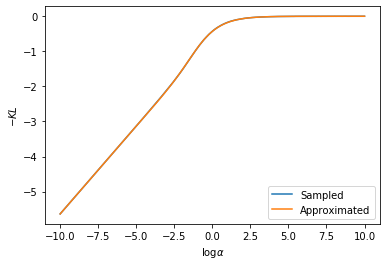
\includegraphics[scale=0.4]{pic/kl-1.png}
			}
			\subfigure[Approximation Deviation with $\log\alpha$]{
				\centering
				\label{fig:exp1-2}			
				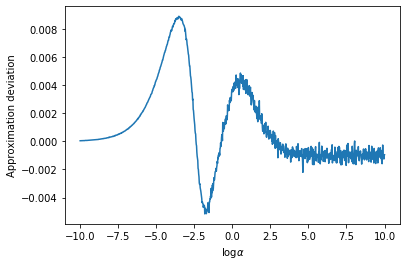
\includegraphics[scale=0.4]{pic/kl-2.png}
			}
			\caption{KL Approximation Curve}
			\label{fig:exp1}
		\end{figure}
	At first, to verify the KL approximation mentioned in Equation \ref{eq5}. We draw the plots Figure \ref{fig:exp1}. The first subfigure is relationship between $log_{\alpha}$ and $-KL$ and the second subfigure is relationship between $\log_{\alpha}$ and approximation deviation. As what we can see from figures, the approximation trick mentioned in paper \cite{molchanov2017variational} is valid.

	\subsubsection{Multi-Layer Perception With Sparse Variational on MNIST}
	On Multi-Layer Perception, we tested sparsity ability of Sparse Variational Dropout, the results show that it achieves a compression of $69.7\%$, and maintains good enough accuracy of $98.4\%$. The change of performance with sparsity under $100$ epochs is as the Figure {\ref{fig:exp2-1}}.
		\begin{figure}[ht]
			\centering
			\subfigure[Training Curve of MLP with SparseVD on MNIST]{
				\centering
				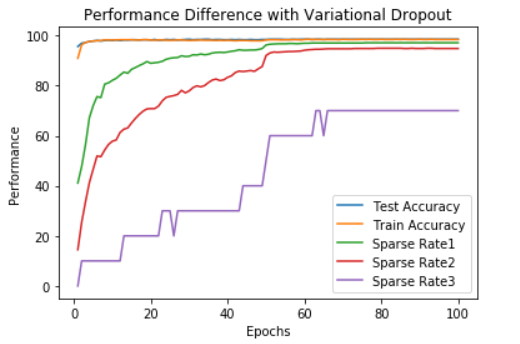
\includegraphics[scale=0.4]{pic/exp2-1.png}
				\label{fig:exp2-1}
			}
			\subfigure[Visualization Sparse Weights on First Layer]{
				\centering
				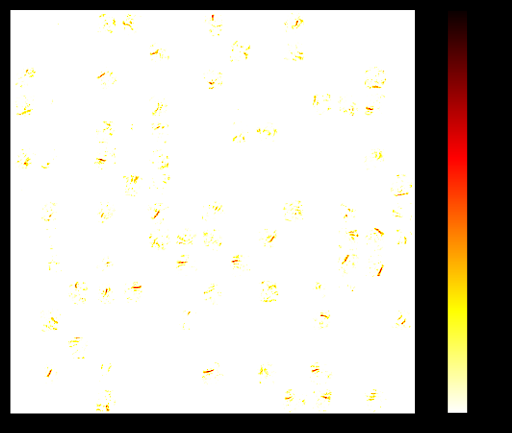
\includegraphics[scale=0.35]{pic/exp2-2.png}
				\label{fig:exp2-2}
			}
			\caption{MLP with SparseVD on MNIST}
			\label{fig:exp2}
		\end{figure}	
	After 63 epochs training, the sparsity stop convergence and achieves $70\%$. We confirmed that the application of SparseVD doesn’t hurt the model accuracy. Three sparse rate curve correspond to all three full connection layers.\\
	In order to make the experiment result more visible, we draw a picture with the weights in first layer after training. The figure shows the obvious compression effect caused by Sparse VD. Red color means weight is large, and white color means weight approach to 0. Obviously, only a small part of weights remains after applying sparse variational dropout.\\

	\subsubsection{AlexNet With Variational Dropout on Cifar-10}
	We tested the performance of AlexNet with Sparse Variational Dropout on Cifar10 dataset.\\
	Orginal Alexnet has accuracy of about $75\%$ on Cifar10 dataset. Though the compression effect is not so obvious as on last MLP model, it also doesn’t hurt the accuracy significantly. The Sparse-1 corresponds to the last full-connection layer, Sparse-2 to the second last full-connection layer, and so on.\\
		\begin{figure}[ht]
			\centering
			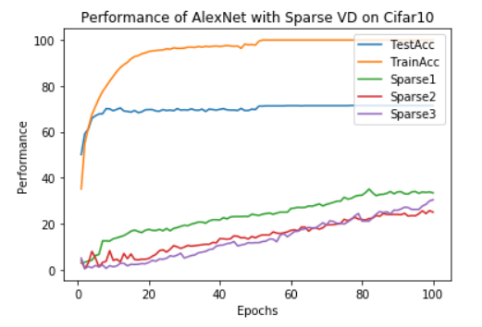
\includegraphics[scale=0.4]{pic/exp3.png}
			\caption{Training Curve of AlexNet with SparseVD on Cifar10}
			\label{fig:exp3}
		\end{figure}\\
	We speculate that the SparseVD has a limitation that when model itself cannot achieves a good prediction, the Sparse VD is hard to generate a good sparsity. In our experiment, AlexNet cannot handle Cifar10 dataset as good as performance on Minst (Accuracy around $99\%$), it just has $70\%$ accuracy on test data. In other way, AlexNet is not suitable for Cifar10 task, thus the Sparse VD are keen to remain more weights because it cannot distinguish whether it's important for specified task or not.\\
	We also notice that the model is motivated to be more sparsified in deeper layers, and we deem the reason is that the features in deeper layer is more abstract, thus the fewer weight will contribute to the final classification.\\

	\subsubsection{LeNet5 With Sparse Varitional Dropout on Randomly Labeled MNIST}
	We tested LeNet-5 with Sparse VD on common Minst dataset, and on $50\%$ randomly labeled Minst dataset. We also tested Lenet-5 with Binary Dropout with dropout rate $0.5$ on randomly labeled Minst dataset as a comparison. After 50 epochs, we got the performance as Figure {\ref{fig:exp4}}
		\begin{figure}[ht]
			\centering
			\subfigure[SVD+MNIST]{
				\centering
				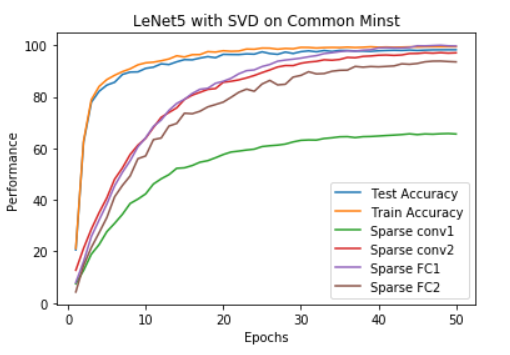
\includegraphics[scale=0.25]{pic/exp4-1.png}
				\label{fig:exp4-1}
			}
			\subfigure[BD+RL-MNIST]{
				\centering
				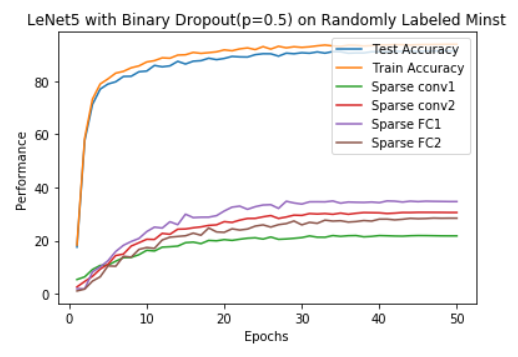
\includegraphics[scale=0.25]{pic/exp4-2.png}
				\label{fig:exp4-2}
			}
			\subfigure[SVD+RL-MNIST]{
				\centering
				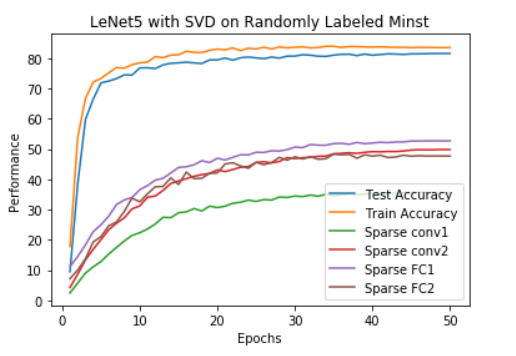
\includegraphics[scale=0.25]{pic/exp4-3.png}
				\label{fig:exp4-3}
			}
			\caption{Training Curve of Lenet-5 On Original and Randomly Labeld MNIST}
			\label{fig:exp4}
		\end{figure}\\

		\begin{table}[!htbp]
			\centering
			\caption{Result}
			\begin{tabular}{ccccccc}
				\toprule
				Model& Train AR& Test AR& Conv1 SR& Conv2 SR& Fc1 SR& Fc2 SR\\
				\midrule
				SVD+MNIST& 99.40& 98.22& 65.56& 97.03& 99.66& 93.53\\
				SVD+RL-MNIST& 83.51& 81.57& 35.58& 49.83& 52.70& 47.70\\ 
				BD+RL-MNIST& 93.93& 91.45& 21.79& 30.60& 34.71& 28.46\\
				\bottomrule
			\end{tabular}
		\end{table}
	The results demonstrates that Sparse VD cannot fit randomly labeled data well, random labeling hurt the model’s prediction ability as well as the sparsity. However, the Binary Dropout performed well on randomly labeled dataset. We give a explanation that the Sparse VD methods decides to drop every single weight and provide a constant prediction, which also means Sparse VD implicitly penalizes memorization and favors generalization.\\

	\subsection{Conclusion}

	Through theoretical analysis and experiments investigation, we confirmed Sparse Variational Dropout's ability of generating obvious sparsity without hurting the accuracy. We tested its performance on Multi-Layer Perceptron and AlexNet. We explained our understanding of the power and limitation of this technique, and implemented the whole computation codes.\\
	As we can see from our experiments, with experiments given by the paper, we can some interesting conclusions as follows.\\
	For different tasks, our method will lead to a very good sparsity on the model suitable enough for the task, but for the model that is not suitable for the task, the effect is not obvious or even worse. This might be the limitation of this algorithm.\\
	To help calculate the gradient conveintly and save the training time, the paper introduce a new loss function with approximation KL divergence as Equation {\ref{eq5}}. However, this is just a numerical approximation function, without reasonable explanation. This is where the assumptions might be hard to interpretate.\\
	In the future, we can focus on giving a better algorithm on interpretable loss function and try to modify the terrible performance on random labeling task.\\
	Fortunately, with sparsifying methods like Sparse VD, we can get more sparse neural networks, which will motivate the research on interpretability of some Deep Neural Networks models like CNNs.\\
	As what we can learn from lectures, Dropout is a cheap trick to save computer resourses and achieve good performance in training deep neural networks in practice. I believe Dropout research might bring great help to Network Architecture Search.\\

	\section{Disccussion}
	From perspective from textbook \cite{shalev2014understanding}. Unnecessary complex structure is not ideal by Occam’s Razor principle. The Sparse Variational Dropout in DNNs is really meaningful because it regularizes the model params effectively, keep the model from overfitting, and make it easier to store and computing.\\
	Futhermore, the idea of constructing a neural network with more sparse weights coincides with the property of sparse signal transmission between neurons in computational neuroscience \cite{1611.06694} in bio-interpretability view. Studying the more sparse neural networks will bring many beneficial parts to the interpretability of neural networks.\\
	Besides the method proposed by this paper, we also have some popular methods to learn sparse neural networks. \cite{louizos2017learning} proposed a way to use $l_0$ regularization to learn sparse neural networks. And \cite{1803.03635} proposed to use pruning methods in neural networks to reduce $90\%$ of parameter counts but not harm accuracy using "Lottery Hypothesis", where Sparse VD has similar effect. However, "Lottery" Pruning also has fatal shortcomings that if we train the model with the structure after pruning, the final convergence cannot be attached, which is against our common sense. Unfortunately, the paper didn’t give a reason for the weird phenomenon.\\
	Moreover, Google did work on comparing some popular sparsifying training methods recently in \cite{gale2019state}. The work compare some popular sparse methods nowadays such as $l_0$ regularization, random pruning, magnitude pruning on resnet-50 and transfomers for some NLP task. They also achieve elegant performance, both accuracy and sparse rate.\\
	We share some code patches in our appendix and submit source code in our supplementary materials, which is written in Pytorch 1.1.0 framework running on CUDA 9.0. However, the source code is not the release version, there might be some bugs. If you have some questions about code, you are welcome to email and discuss to authors of this report.\\

\clearpage

\bibliographystyle{unsrt}
\bibliographystyle{plain}
\bibliography{ref}

\clearpage

\appendixpage

\begin{appendices}
	\section{Code Patches}
		\begin{python}
# define LinearSVDO Layer
class LinearSVDO(nn.Module):
    def __init__(self, in_features, out_features, threshold, bias=True):
        super(LinearSVDO, self).__init__()
        self.in_features = in_features
        self.out_features = out_features
        self.threshold = threshold

        self.W = Parameter(torch.Tensor(out_features, in_features))
        self.log_sigma = Parameter(torch.Tensor(out_features, in_features))
        self.bias = Parameter(torch.Tensor(1, out_features))
        
        self.reset_parameters()

    def reset_parameters(self):
        self.bias.data.zero_()
        self.W.data.normal_(0, 0.02)
        self.log_sigma.data.fill_(-5)        
        
    def forward(self, x):
        self.log_alpha = self.log_sigma * 2.0 - 2.0 * torch.log(1e-16 + torch.abs(self.W))
        self.log_alpha = torch.clamp(self.log_alpha, -10, 10) 
        
        if self.training:
            lrt_mean =  F.linear(x, self.W) + self.bias
            lrt_std = torch.sqrt(F.linear(x * x, torch.exp(self.log_sigma * 2.0)) + 1e-8)
            eps = lrt_std.data.new(lrt_std.size()).normal_()
            return lrt_mean + lrt_std * eps
    
        return F.linear(x, self.W * (self.log_alpha < 3).float()) + self.bias
        
    def kl_reg(self):
        # Return KL here -- a scalar 
        k1, k2, k3 = torch.Tensor([0.63576]), torch.Tensor([1.8732]), torch.Tensor([1.48695])
        kl = k1 * torch.sigmoid(k2 + k3 * self.log_alpha) - 0.5 * torch.log1p(torch.exp(-self.log_alpha))
        a = - torch.sum(kl)
        return a
        \end{python}

\clearpage

        \begin{python}
# Define New Loss Function -- SGVLB 
class SGVLB(nn.Module):
    def __init__(self, net, train_size):
        super(SGVLB, self).__init__()
        self.train_size = train_size
        self.net = net

    def forward(self, input, target, kl_weight=1.0):
        assert not target.requires_grad
        kl = 0.0
        for module in self.net.children():
            if hasattr(module, 'kl_reg'):
                kl = kl + module.kl_reg()
        return F.cross_entropy(input, target) * self.train_size + kl_weight * kl
		\end{python}

\end{appendices}

\end{document}














